\newcommand{\doctitle}{Numerical Methods Problem Sheet 1}
\providecommand{\doctitle}{Not Untitled}
\providecommand{\docauthor}{Nicolas Hafner}
\providecommand{\doccopyright}{Shirakumo}

\documentclass[12pt,a4paper,titlepage]{article}
\usepackage[utf8]{inputenc}
\usepackage[T1]{fontenc}
\usepackage[top=1.5cm, bottom=2.5cm, left=1cm, right=1cm]{geometry}
\usepackage{textcomp}
\usepackage{amsmath}
\usepackage{amsfonts}
\usepackage{amssymb}
\usepackage{amsthm}
\usepackage{fancyhdr}
\usepackage{fix-cm}
\usepackage{graphicx}
\usepackage{hyperref}
\usepackage{xcolor}
\usepackage{listings}
\usepackage{float}
\usepackage{wrapfig}
\usepackage{datetime}
\usepackage{enumitem}
\usepackage{minted}
\usepackage{epstopdf}

\newdateformat{dmny}{\monthname[\THEMONTH] \THEYEAR}
\newdateformat{dyo}{\THEYEAR}
\setlength{\headheight}{30pt}
\pagestyle{fancy}

\title{\doctitle}
\author{\docauthor}
\date{\d_mny\today}

\lhead{\docauthor}
\chead{\doctitle}
\lfoot{\copyright \dyo\today\; \doccopyright}
\cfoot{\thepage\ / \pageref{LastPage}}
\rhead{\dmny\today}

\definecolor{mintedbg}{rgb}{0.2,0.2,0.2}
\usemintedstyle{monokai}
\newmintedfile[matlabcode]{matlab}{
  bgcolor=mintedbg, fontfamily=tt,   linenos=true,     numberblanklines=true,
  numbersep=12pt,   numbersep=5pt,   gobble=0,         frame=leftline,
  framerule=0.4pt,  framesep=2mm,    funcnamehighlighting=true,
  tabsize=4,        obeytabs=false,  mathescape=false, samepage=false,
  showspaces=false, showtabs =false, texcl=false,
}

\newmintedfile[cppcode]{cpp}{
  bgcolor=mintedbg, fontfamily=tt,   linenos=true,     numberblanklines=true,
  numbersep=12pt,   numbersep=5pt,   gobble=0,         frame=leftline,
  framerule=0.4pt,  framesep=2mm,    funcnamehighlighting=true,
  tabsize=4,        obeytabs=false,  mathescape=false, samepage=false,
  showspaces=false, showtabs =false, texcl=false,
}

\renewcommand{\thesubsection}{\thesection.\alph{subsection}}


%%% Local Variables:
%%% mode: latex
%%% End:


\begin{document}
\begin{center}{\bfseries\Huge\doctitle}\end{center}

\section{Problem 1}
\subsection{}

$$ \left(\begin{array}{ccccc}
     d_1 & 0 & \hdots & 0 & a_1 \\
     0 & d_2 & \ddots & \vdots & a_2 \\
     \vdots & \ddots & \ddots & 0 & \vdots \\
     0 & \hdots & 0 & d_{n-1} & a_{n-1} \\
     a_1 & a_2 & \hdots & a_{n-1} & d_n
\end{array}\right) $$

\subsection{}

We are creating a Matrix $A$ of $n^2$ size. The matrix is then cubed, which is at worst an $O(n^3)$ operation. At smaller sizes constant overhead is going to dominate, explaining the divergence from $n^3$.

\subsection{}

\matlabcode{../arrowmatvec2.m}

\subsection{}

Since we just perform two Matrix multiplications with a vector we get a complexity of $O(n^2)$.

\subsection{}

\begin{figure}[H]
  \centering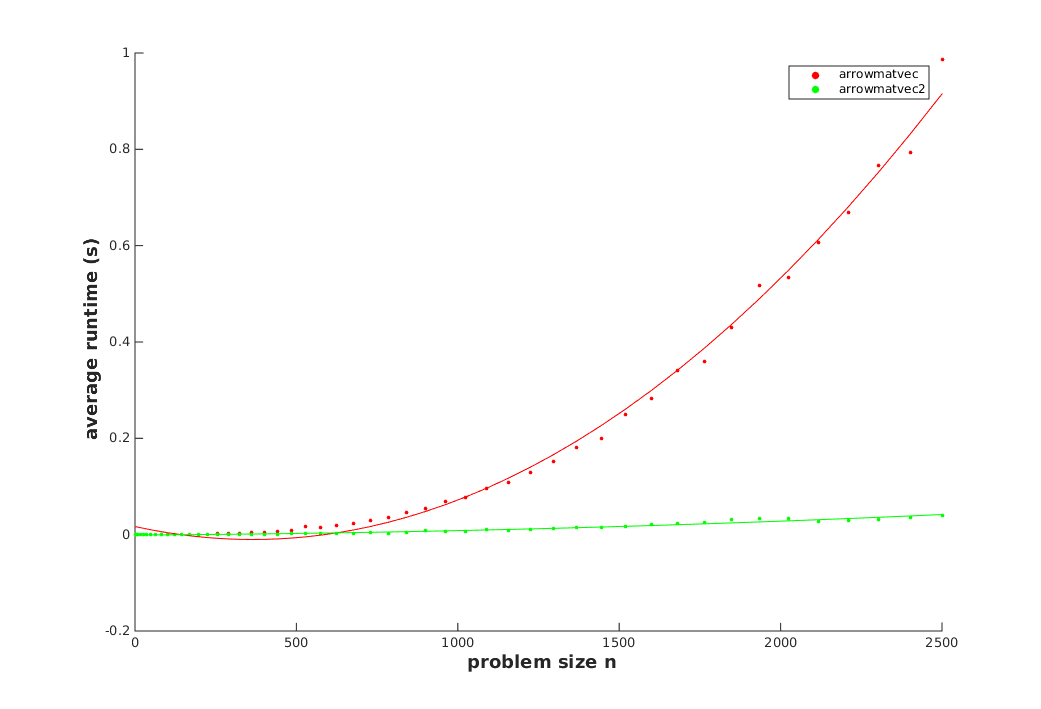
\includegraphics[scale=0.65]{./e1e.png}
\end{figure}

\subsection{}

\cppcode{../e1.cpp}

\section{Problem 2}
\subsection{}
$$ f_1(x_0,h) := \sin(x_0+h)-\sin(x_0) $$
$$ f_2(x_0,h) := 2\cos(x_o+h)\sin\left(\frac{h}{2}\right) $$
$$ \frac{\sin(x_0+h)-\sin(x_0)}{h} = \frac{2\cos(x_0+h)\sin\left(\frac{h}{2}\right)}{h} $$

\begin{figure}[H]
  \centering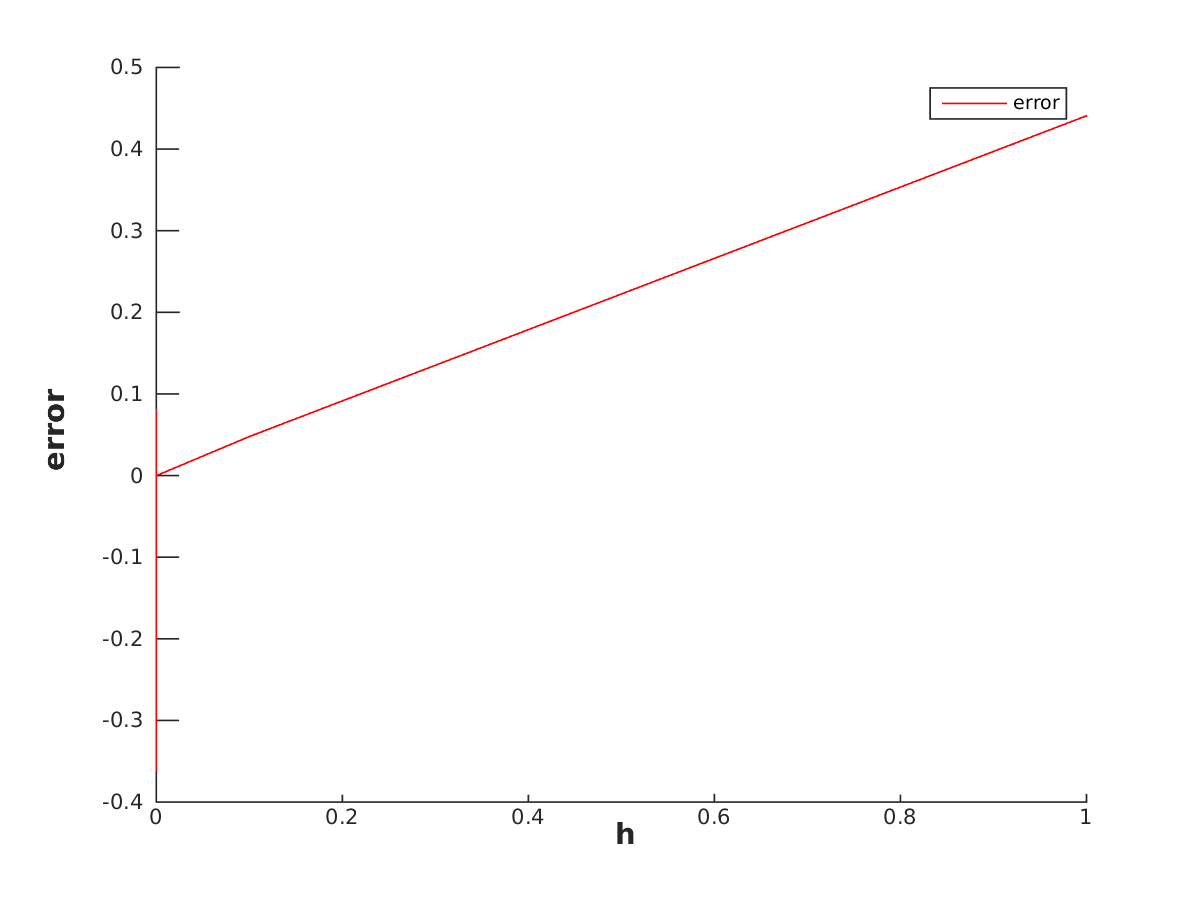
\includegraphics[scale=0.8]{./e2a.png}
\end{figure}

As we cannot calculate the sine exactly and instead need to approximate it, there will always be an error in the result. Thus, subtracting two sines will result in the cancellation phenomenon, increasing the relative error. Avoiding the subtraction will yield a more accurate result.

\subsection{}
$$ \ln(x-\sqrt{x^2-1}) = \ln\left((x-\sqrt{x^2-1})\frac{x+\sqrt{x^2-1}}{x+\sqrt{x^2-1}}\right) = \ln\left(\frac{-1}{x+\sqrt{x^2-1}}\right) = -\ln(x+\sqrt{x^2-1}) $$

Even slight deviation from $0$ ($\sim x\notin [0.003,1.5]$) will result in differences between the two formula. \\

Again, the square root is an approximate function in cases where the number is not a known square, resulting in an error. Cancellation will amplify this error.

\subsection{}
$$ \sqrt{x+\frac{1}{x}}-\sqrt{x-\frac{1}{x}} = (..-..)\frac{..+..}{..+..} = \frac{x+\frac{1}{x}-x+\frac{1}{x}}{..+..} = \frac{2}{\sqrt{x^3+x}+\sqrt{x^3-x}} $$

Square roots and addition of numbers with large exponent differences will result in errors. By changing the formula up, both of these problems can be avoided.

\end{document}

%%% Local Variables:
%%% mode: latex
%%% TeX-master: t
%%% TeX-engine: luatex
%%% TeX-command-extra-options: "-shell-escape"
%%% End:
